% System Architecture Diagram using TikZ
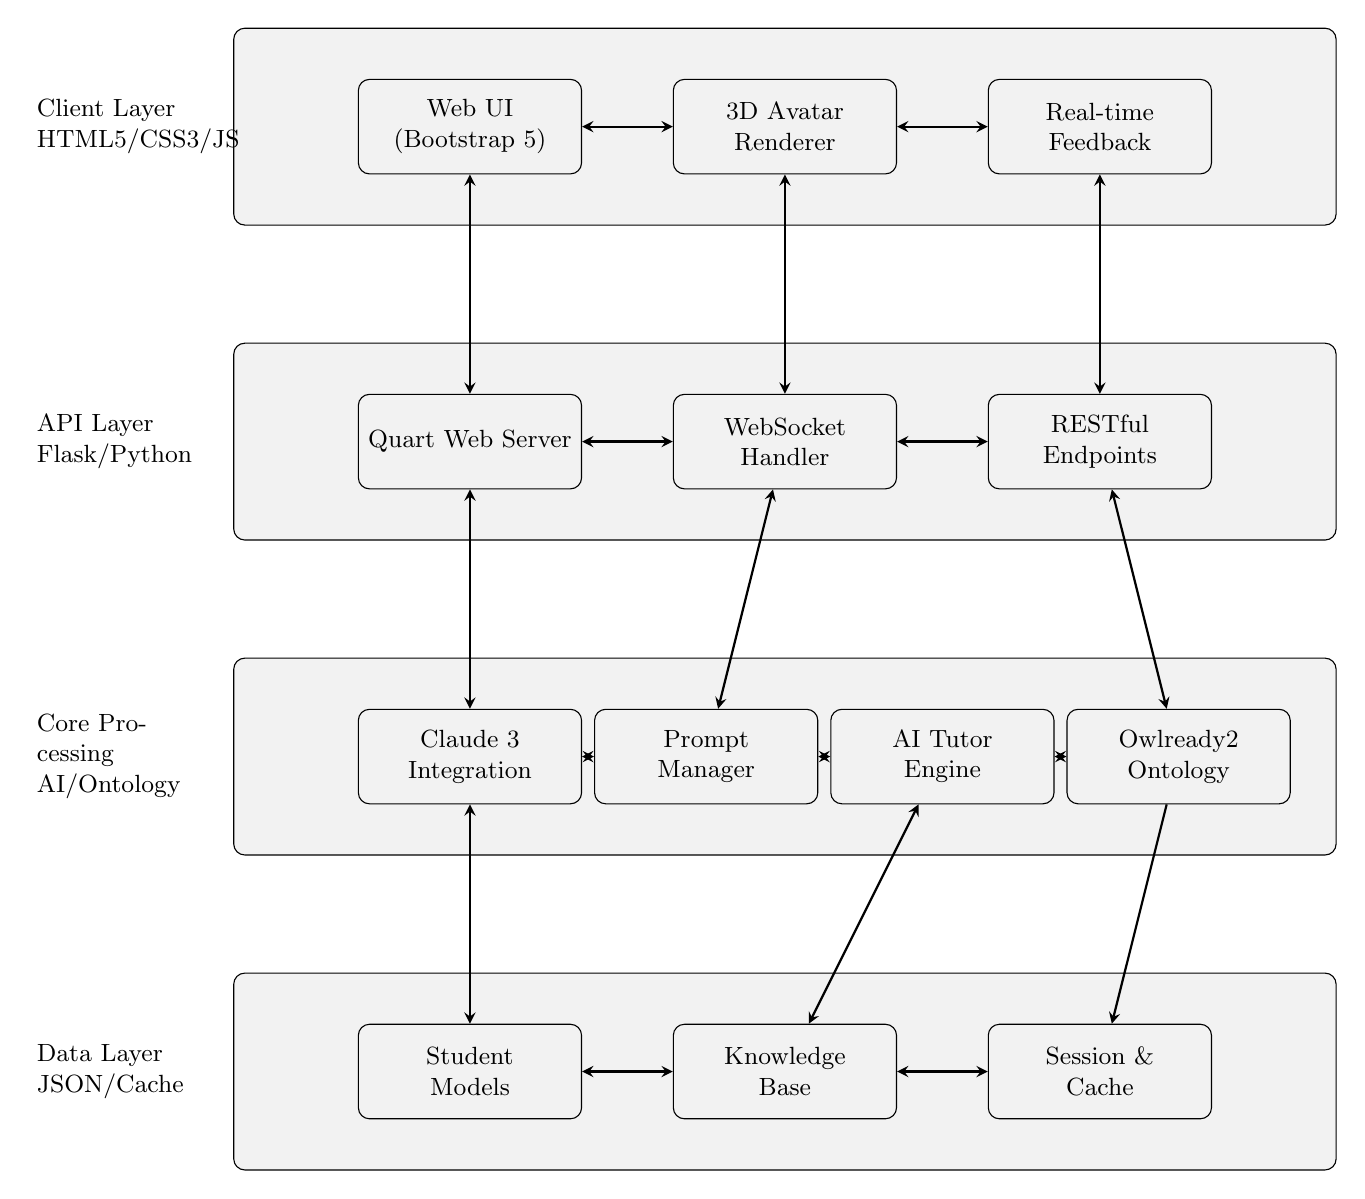
\begin{tikzpicture}[
    % Define styles for different node types
    box/.style={
        draw,
        rectangle,
        rounded corners,
        minimum width=2.8cm,
        minimum height=1.2cm,
        text centered,
        text width=2.6cm,
        font=\small
    },
    layer/.style={
        draw,
        rectangle,
        rounded corners,
        minimum width=14cm,
        minimum height=2.5cm,
        fill=gray!10
    },
    arrow/.style={
        ->,
        >=stealth,
        thick
    },
    bidirectional/.style={
        <->,
        >=stealth,
        thick
    },
    layer_label/.style={
        text width=3cm,
        align=left,
        font=\small
    }
]

% Define the layers with proper spacing
\begin{scope}[shift={(0,0)}]
    % Layer background rectangles with adjusted spacing
    \node[layer] (client) at (0,12) {};
    \node[layer] (api) at (0,8) {};
    \node[layer] (core) at (0,4) {};
    \node[layer] (data) at (0,0) {};

    % Layer labels on the left with better spacing
    \node[layer_label] at (-8,12) {Client Layer\\HTML5/CSS3/JS};
    \node[layer_label] at (-8,8) {API Layer\\Flask/Python};
    \node[layer_label] at (-8,4) {Core Pro-\\cessing\\AI/Ontology};
    \node[layer_label] at (-8,0) {Data Layer\\JSON/Cache};

    % Client Layer Components with even spacing
    \node[box] (browser) at (-4,12) {\parbox{2.6cm}{\centering Web UI\\(Bootstrap 5)}};
    \node[box] (avatar) at (0,12) {\parbox{2.6cm}{\centering 3D Avatar\\Renderer}};
    \node[box] (frontend) at (4,12) {\parbox{2.6cm}{\centering Real-time\\Feedback}};

    % API Layer Components
    \node[box] (gateway) at (-4,8) {Quart Web Server};
    \node[box] (websocket) at (0,8) {\parbox{2.6cm}{\centering WebSocket\\Handler}};
    \node[box] (endpoints) at (4,8) {\parbox{2.6cm}{\centering RESTful\\Endpoints}};

    % Core Processing Components with adjusted spacing
    \node[box] (llm) at (-4,4) {\parbox{2.6cm}{\centering Claude 3\\Integration}};
    \node[box] (prompt) at (-1,4) {\parbox{2.6cm}{\centering Prompt\\Manager}};
    \node[box] (tutor) at (2,4) {\parbox{2.6cm}{\centering AI Tutor\\Engine}};
    \node[box] (ontology) at (5,4) {\parbox{2.6cm}{\centering Owlready2\\Ontology}};

    % Data Layer Components
    \node[box] (student) at (-4,0) {\parbox{2.6cm}{\centering Student\\Models}};
    \node[box] (knowledge) at (0,0) {\parbox{2.6cm}{\centering Knowledge\\Base}};
    \node[box] (session) at (4,0) {\parbox{2.6cm}{\centering Session \&\\Cache}};

    % Vertical Connections
    \draw[bidirectional] (browser) -- (gateway);
    \draw[bidirectional] (avatar) -- (websocket);
    \draw[bidirectional] (frontend) -- (endpoints);

    \draw[bidirectional] (gateway) -- (llm);
    \draw[bidirectional] (websocket) -- (prompt);
    \draw[bidirectional] (endpoints) -- (ontology);

    \draw[bidirectional] (llm) -- (student);
    \draw[bidirectional] (tutor) -- (knowledge);
    \draw[arrow] (ontology) -- (session);

    % Horizontal Connections
    \draw[bidirectional] (browser) -- (avatar);
    \draw[bidirectional] (avatar) -- (frontend);
    \draw[bidirectional] (gateway) -- (websocket);
    \draw[bidirectional] (websocket) -- (endpoints);
    \draw[bidirectional] (llm) -- (prompt);
    \draw[bidirectional] (prompt) -- (tutor);
    \draw[bidirectional] (tutor) -- (ontology);
    \draw[bidirectional] (student) -- (knowledge);
    \draw[bidirectional] (knowledge) -- (session);
\end{scope}
\end{tikzpicture} 